% !TEX TS-program = pdflatex
% !TEX encoding = UTF-8 Unicode



\documentclass[11pt,a4paper]{article}

%\usepackage[francais]{babel} % bug à la compilation chez moi
\usepackage[T1]{fontenc}
\usepackage[utf8]{inputenc}

\usepackage{amsmath,amsfonts,amssymb}

\usepackage{geometry}
\geometry{margin=75pt}

\usepackage[upright]{fourier}
\usepackage{subfig}

\usepackage{shadethm}

\usepackage{color}
\definecolor{gris_clair}{gray}{.9}
\definecolor{gris}{gray}{.35}
\definecolor{vert}{rgb}{0,0.5,0}
\definecolor{rouge}{rgb}{0.5,0,0}
\definecolor{turquoise}{rgb}{0,0.5,0.5}

\usepackage{listings}
\usepackage{paralist}
\usepackage{stmaryrd} % bug à la compilation chez moi[Matthias]
\usepackage{tikz}
\usetikzlibrary{shapes.multipart}
\usetikzlibrary{calc}

\lstset{
language=Python,
backgroundcolor=\color{gris_clair},
frame=single,
basicstyle=\footnotesize\ttfamily\color{gris},
identifierstyle=\color{black},
keywordstyle=\color{vert},
stringstyle=\color{rouge}, showstringspaces=false,
commentstyle=\itshape\color{turquoise},
%numbers=left, numbersep=5pt, numberstyle=\color{gris}\tiny,stepnumber=5,
breaklines=true,
literate=
  {é}{{\'e}}1 {É}{{\'E}}1 {à}{{\`a}}1 {è}{{\`e}}1% 
  {À}{{\`A}}1 {È}{{\'E}}1 {ë}{{\"e}}1 {ï}{{\"i}}1%
  {â}{{\^a}}1 {ê}{{\^e}}1 {î}{{\^i}}1 {ô}{{\^o}}1% 
  {û}{{\^u}}1 {Â}{{\^A}}1 {Ê}{{\^E}}1 {Î}{{\^I}}1%
  {Ô}{{\^O}}1 {œ}{{\oe}}1 {Œ}{{\OE}}1 {æ}{{\ae}}1%
  {Æ}{{\AE}}1 {ç}{{\c c}}1 {Ç}{{\c C}}1 {€}{{\EUR}}1 ,
morekeywords={len,input,range}}         


\title{Correction des exercices sur le labyrinthe}
\date{}
\author{Antonin Dudermel \and Ambroise Poulet \and Matthias Goffette}

\begin{document}

\newshadetheorem{defin}{Définition}
\newshadetheorem{theo}{Théorème}

\maketitle

\begin{it}
On propose un algorithme créant un labyrinthe parfait de dimension $n$. Nous voulons le modifier, d'abord pour enegistrer le labyrinthe en une image, puis pour construire le chemin entre les cases $(0,0)$ et $(n-1,n-1)$.
\end{it}

\section{Création de l'image}

On va représenter le labyrinthe de taille $n\times n$ par une image de $(2n+1)\times (2n+1)$ pixels. Les zones praticables seront représentées en blanc, les zones non-praticables en noir. Alors :
\begin{itemize}
	\item Une case du labyrinthe $\mathtt{atteinte[i,j]}, ~ (i,j) \in \llbracket 0,n \llbracket ^2$, est représentée par le pixel $(2i+1,2j+1)$, ce pixel est toujours blanc. Par exemple, sur la figure \ref{qc}, la case b $(1,0)$ est représentée par le pixel de coordonnées $(3,1)$. De même pour les cases a,b et d
	\item Comme on ne peut pas se déplacer en diagonale, les pixels diagonaux, de coordonnées $(2k,2l), ~ (k,l) \in \llbracket 0,n \llbracket ^2 $, sont toujours noirs.
	\item 
		Soient deux cases adjacentes $p$ et $q$. Remarquons tout d'abord que le pixel se trouvant entre celui représentant $p$ et celui représentant $q$ a pour coordonnées $(\dfrac{x_p+x_q}{2},\dfrac{y_p+y_q}{2})$ (1,2,3 et 4 sur la figure \ref{qc}). 
	\begin{itemize}
		\item {\itshape Si} on peut se déplacer de $p$ à $q$, par exemple entre a et b dans la figure \ref{expl}, 

	\end{itemize}
\end{itemize}


\begin{figure}[h]
\begin{center}

\hfill
\subfloat[quatre cases]{
\label{qc}
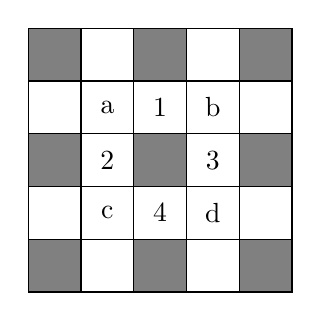
\begin{tikzpicture}[scale=0.67]
	\draw (0,0) grid (5,5);
	\foreach \i in {0,2,4}
		{\foreach \j in {0,2,4}
			{\draw[color=black,fill=gray] (\i,\j)--++(0,1)--++(1,0)--++(0,-1)--cycle;};
	};
	\draw (1,3) ++ (0.5,0.5) node {a};
	\draw (3,3) ++ (0.5,0.5) node {b};
	\draw (1,1) ++ (0.5,0.5) node {c};
	\draw (3,1) ++ (0.5,0.5) node {d};
	\draw (2,3) ++ (0.5,0.5) node {1};
	\draw (1,2) ++ (0.5,0.5) node {2};
	\draw (3,2) ++ (0.5,0.5) node {3};
	\draw (2,1) ++ (0.5,0.5) node {4};	
\end{tikzpicture}
}
\hfill
\subfloat[exemple]{
\label{expl}
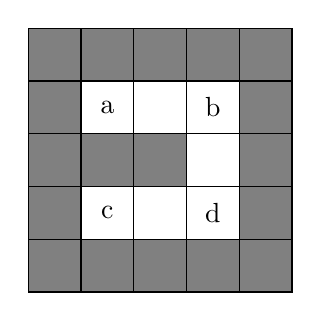
\begin{tikzpicture}[scale=0.67]
	\draw (0,0) grid (5,5);
	\foreach \i in {0,2,4}
		{\foreach \j in {0,2,4}
			{\draw[color=black,fill=gray] (\i,\j)--++(0,1)--++(1,0)--++(0,-1)--cycle;};
	};
	\draw (1,3) ++ (0.5,0.5) node {a};
	\draw (3,3) ++ (0.5,0.5) node {b};
	\draw (1,1) ++ (0.5,0.5) node {c};
	\draw (3,1) ++ (0.5,0.5) node {d};
	%\draw (2,3) ++ (0.5,0.5) node {1};
	\draw[color=black,fill=gray] (1,2)--++(0,1)--++(1,0)--++(0,-1)--cycle;
	%\draw (3,2) ++ (0.5,0.5) node {3};
	%\draw[color=black,fill=gray] (2,1)--++(0,1)--++(1,0)--++(0,-1)--cycle;
	\foreach \i in {1,3}
		{\foreach \j in {0,4}
			{\draw[color=black,fill=gray] (\i,\j)--++(0,1)--++(1,0)--++(0,-1)--cycle;
			 \draw[color=black,fill=gray] (\j,\i)--++(0,1)--++(1,0)--++(0,-1)--cycle;
			};
	};
\end{tikzpicture}
}
\hfill \hbox{}
\caption{Représentation d'une case}

\end{center}
\end{figure}


\subsection{dessin du labyrinthe}

Nous allons réaliser l'enregistrement du labyrinthe au format PGM. Ce format permet d'enegistrer facilement des images en nivau de gris. Définissons donc les couleurs des pixels :

\lstinputlisting[firstline=140,lastline=141]{labyrinthe.py}

\par
En premier lieu, il faut compléter la fonction labyrinthe, en ajoutant un tableau $\mathtt{lislab}$, de dimension $(2n+1) \times (2n+1)$ qui contiendra la représentation du labyrinthe. Le tableau étant par défaut tout noir, on commence par le préremplir en blanchissant les pixels représentant les cases.

\lstinputlisting[firstline=77,lastline=81]{labyrinthe.py}

Il faut ensuite lier les cases entre elles lors de la création du labyrinthe. On remarque de manière astucieuse, que pour deux cases $(x,y)$ et $(x',y')$ adjacentes, le pixel entre les pixels les représentant a pour coordonnées $(x+x'+1,y+y'+1)$. Le code suivant permet donc de faire ce lien.

\lstinputlisting[firstline=102,lastline=104]{labyrinthe.py}

Il suffit alors de retourner le tableau de pixels à la fin de la fonction : la fonction $\mathtt{save\_lab}$ se contente ensuite de sauvegarder le labyrinthe au format désiré.

\lstinputlisting[firstline=145,lastline=155]{labyrinthe.py}


\section{Obtention du chemin}

\subsection{une remarque astucieuse}
La question suivante consiste à construire à la volée le chemin reliant les cases $(0,0)$ et $(n-1,n-1)$.  Le point clé de cette question réside dans les trois lignes suivantes :
\lstinputlisting[linerange={95-96,122-123}]{labyrinthe.py}
On se rend alors compte qu'on n'ajoute jamais à la pile qu'une case adjacente à la case du sommet de la pile. Ainsi, si l'état de la pile est \ref{pilek}, alors les cases $C_{k-1}$ et $C_{k}$ sont adjacentes ; le chemin de $C_{k-1}$ à $C_{k}$ est alors $[C_{k-1},C_{k}]$. Par récurrence, si la pile est comme représenté en \ref{pilefin}, alors Le chemin allant de $C_0$ à $C_n$ est exactement l'ensemble des cases contenues dans la pile. Or $C_0$ est la case $(0,0)$. Ainsi, en appliquant ce résultat pour $C_n = (n-1,n-1)$, si $\mathtt{cellule}$ contient $(n-1,n-1)$, alors $\mathtt{pile}$ contient le chemin allant de $(0,0)$ à $(n-1,n-1)$.

\begin{figure}[h]
	\begin{center}

\subfloat[Pile $k$]{
\label{pilek}
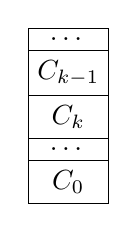
\begin{tikzpicture}[stack/.style={rectangle split, rectangle split parts=#1,draw, anchor=center}]
        \node[stack=5] {
        \nodepart{one}$\dots$
        \nodepart{two}$C_{k-1}$
        \nodepart{three}$C_{k}$
        \nodepart{four}$\dots$
        \nodepart{five}$C_0$
};
\end{tikzpicture}
}
\hspace{2cm}
\subfloat[Pile à l'arrivée]{ 
\label{pilefin}
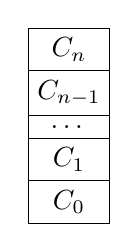
\begin{tikzpicture}[stack/.style={rectangle split, rectangle split parts=#1,draw, anchor=center}]
        \node[stack=5]  {
        \nodepart{one}$C_n$
        \nodepart{two}$C_{n-1}$
        \nodepart{three}$\dots$
        \nodepart{four}$C_1$
        \nodepart{five}$C_0$
};
\end{tikzpicture}
}
	\caption{divers états de la pile}
	\end{center}
\end{figure}

\subsection{implantation}

Il s'agit donc simplement de faire une copie de la pile, sans modifier cette dernière, quand le sommet de la pile vaut $(n-1,n-1)$. Le code suivant permet de copier une version renversée de la pile. Le principe est simple : en appelant $\mathtt{revdup(p)}$, on dépile les éléments de $\mathtt{p}$ pour les empiler dans deux piles : on utilise l'une pour reconstituer p, et on retourne l'autre.\\

\lstinputlisting[firstline=30,lastline=42]{labyrinthe.py}

On a donc besoin d'une pile $\mathtt{chemin}$, qui contiendra le chemin à la fin. Il suffit ensuite de recopier la pile dans $\mathtt{chemin}$ au bon moment, puis de tracer le chemin dans le tableau de pixels :

\lstinputlisting[firstline=92,lastline=95]{labyrinthe.py}
\lstinputlisting[firstline=127,lastline=133]{labyrinthe.py}

\begin{figure}[p]
\begin{center}
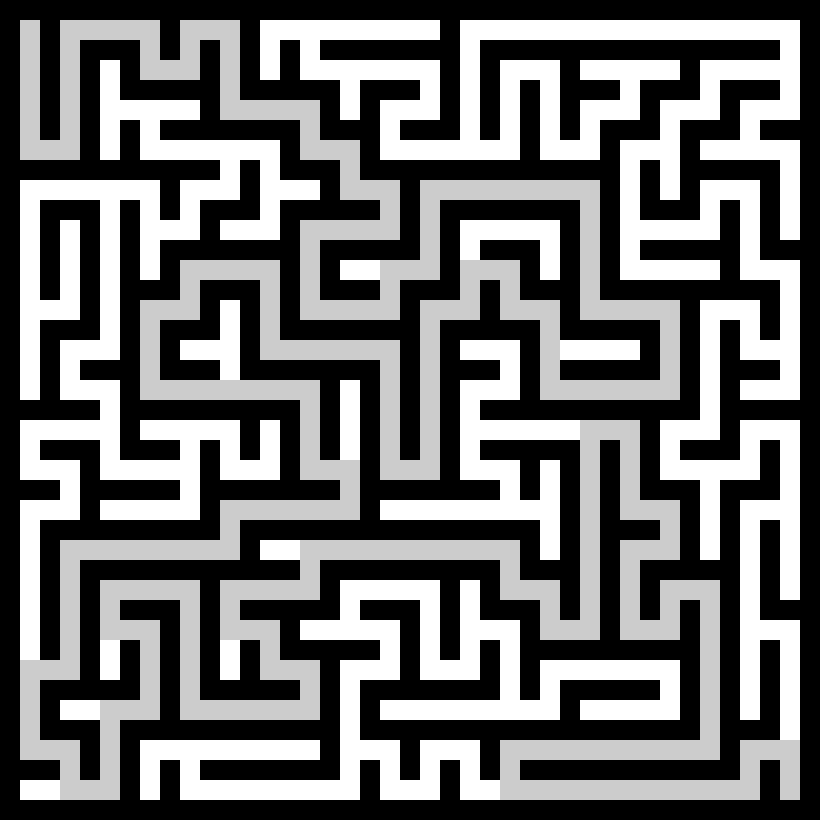
\includegraphics[scale=0.4]{laby.png}
\caption{le labyrinthe}
\end{center}
\end{figure}
\end{document}